\section{Evaluation}
We measure result based on two metrics, objective and subjective metrics as shown in Figure \ref{fig:objectiveMetrics} and \ref{fig:subjectiveMetrics}. 
\begin{figure}
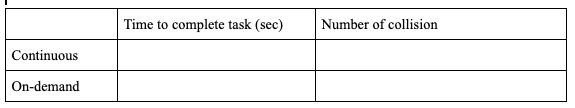
\includegraphics[width=8cm]{img/objectivemetrics.png}
\caption{Objective Metrics}
\label{fig:objectiveMetrics}
\end{figure}
\begin{figure}
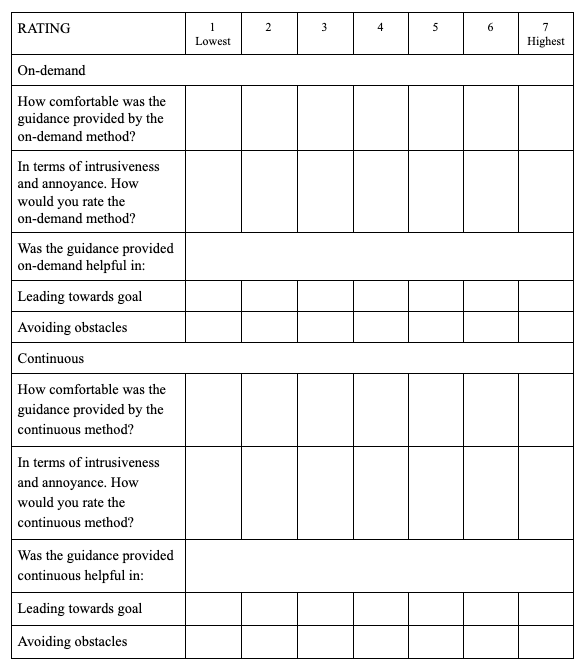
\includegraphics[width=8cm]{img/subjectivemetrics.png}
\caption{Subjective Metrics}
\label{fig:subjectiveMetrics}
\end{figure}
We were not able to get data for subjective metrics due to COVID-19. 
Furthermore, the extent to which we can gather objective data will also be limited. 
If and when we are able to perform the experiment in lab, one important factor to take into consideration is that the response of blindfolded people with perfect vision and people who are visually impaired might be different. 
People who are blindfolded might get more nervous or respond differently when navigating through the environment which might lead to bias is result. 
It would be preferable to test the algorithm with originally visually-impaired subjects. 
However in its current state, the algorithm is not complete and safe for implementation. 

Additionally, since the experiment is running in simulation, there are certain parameters that cannot be fully evaluated. 
For instance, it is not possible to measure the total duration of navigation with on-demand and continuous guidance, since we cannot account for the human arm travel duration in the former case. 
All that can be extracted from the simulation is duration to determine the motion plan. 
It is also not possible to determine if, even after determining the motion plan, there will be any collisions between obstacles and the human. 
% \setlength{\belowcaptionskip}
\begin{figure}
    \centering
    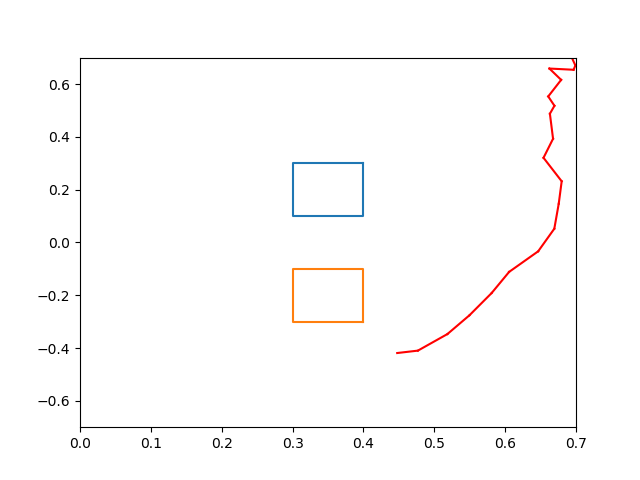
\includegraphics[width = \linewidth]{img/continuous_30s03ms.png}
    \caption{Trajectory for continuous guidance - duration 30s 3ms}
    \label{fig:ContinuousGuidance}
\end{figure}
\begin{figure}
    \centering
    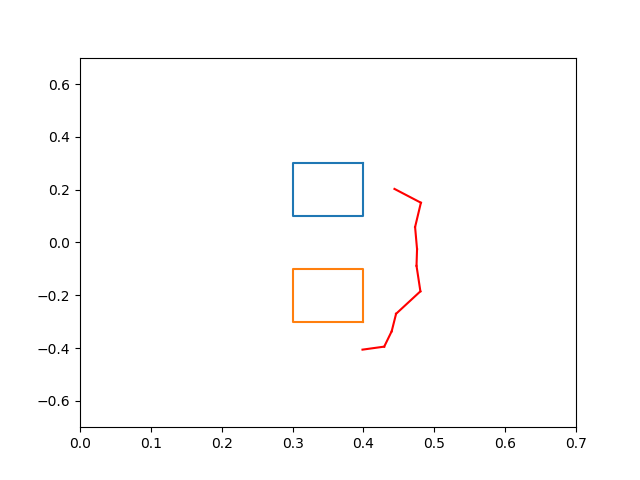
\includegraphics[width = \linewidth]{img/ondemand_18s03ms.png}
    \caption{Trajectory for on-demand guidance - duration 18s 4ms}
    \label{fig:OndemandGuidance}
\end{figure}
In the case of continuous and on-demand guidance, an example trajectory is shown in Figure \ref{fig:ContinuousGuidance} and \ref{fig:OndemandGuidance}. 
It is an obvious find that the continuous guidance motion plan had a longer duration as opposed to the on-demand plan, since the distance over which the trajectory is planned is longer. 
The duration for the motion plan with continuous guidance was 30s 3ms, and with on-demand guidance it was 18s 4ms. 
Note how the trajectory ensures that human arm does not collide with the obstacles in the workspace. 
However, also note that the issue which was brought up before about the stringency of the human arm conscious cost function is evident in the results. 
As the trajectory moves beyond the obstacles, the cost function, which does not consider the flexibility of the human arm, starts to limit exploration. 

Furthermore, because of the heuristic in the A* algorithm, the graph traversal is excessively greedy and can sometimes take a path towards the goal which results in a position that is disadvantageous for the human, although it is still closer to the goal. 
Possible methods to improve the strategy are discussed in the discussion section.  
